% =====================================================================
%  TFPT --- Origin Theory
%  The seam as a horizon, the cyclic compiler hull, and the
%  self-reproducing parameter-free fixed point.
%  [I]/[L] structural core (v53-v56) + honestly-typed [P] interpretation.
% =====================================================================
\documentclass[11pt,a4paper]{article}
\usepackage[T1]{fontenc}
\usepackage[utf8]{inputenc}
\usepackage[english]{babel}
\usepackage{lmodern}
\usepackage[a4paper,margin=2.3cm]{geometry}
\usepackage{amsmath,amssymb,amsthm,mathtools}
\usepackage{booktabs,array,tabularx}
\usepackage{enumitem}
\usepackage{xcolor}
\usepackage{graphicx}
\usepackage{tikz}
\usetikzlibrary{arrows.meta,positioning,calc,decorations.pathmorphing}
\usepackage[most]{tcolorbox}
\usepackage{microtype}
\usepackage[hidelinks,colorlinks=true,linkcolor=blue!55!black,urlcolor=blue!55!black]{hyperref}
\emergencystretch=3em
\graphicspath{{figures/}}

\definecolor{tfblue}{HTML}{1F4E79}
\definecolor{tfgreen}{HTML}{1E7B45}
\definecolor{tfred}{HTML}{9B2226}
\definecolor{tfgold}{HTML}{B8860B}

\newtcolorbox{keybox}[1][]{enhanced,breakable,colback=tfblue!5!white,colframe=tfblue,fonttitle=\bfseries,coltitle=white,title={#1}}
\newtcolorbox{winbox}[1][]{enhanced,breakable,colback=tfgreen!6!white,colframe=tfgreen!75!black,fonttitle=\bfseries,coltitle=white,title={#1}}
\newtcolorbox{gapbox}[1][]{enhanced,breakable,colback=tfred!5!white,colframe=tfred!80!black,fonttitle=\bfseries,coltitle=white,title={#1}}
\newtcolorbox{intbox}[1][]{enhanced,breakable,colback=tfgold!7!white,colframe=tfgold!80!black,fonttitle=\bfseries,coltitle=white,title={#1}}

% --- six-grade status markers ---
\newcommand{\tI}{{\small\textcolor{tfgreen}{\textbf{[I]}}}}
\newcommand{\tL}{{\small\textcolor{tfblue}{\textbf{[L]}}}}
\newcommand{\tF}{{\small\textcolor{tfgreen!45!black}{\textbf{[F]}}}}
\newcommand{\tN}{{\small\textcolor{tfgreen}{\textbf{[N]}}}}
\newcommand{\tP}{{\small\textcolor{tfgold}{\textbf{[P]}}}}
\newcommand{\tA}{{\small\textcolor{tfred}{\textbf{[A]}}}}
\newcommand{\markerkey}{\par\vspace{1.5pt}\noindent{\scriptsize\itshape\textcolor{black!58}{Marker key:\ \tI~exact identity\,$\cdot$\,\tL~Lie/lattice theorem\,$\cdot$\,\tN~numerical fixed point\,$\cdot$\,\tP~physical/interpretive\,$\cdot$\,\tA~open.}}\par\vspace{2pt}}
\newcommand{\veri}[1]{\,{\footnotesize\textcolor{tfblue!70!black}{[\,\texttt{verification/#1}\,]}}}
% falsifier-class tags (Alessandro: which falsifier tests what)
\newcommand{\fcore}{{\small\textcolor{tfgreen!50!black}{\textbf{[core]}}}}
\newcommand{\fcyc}{{\small\textcolor{tfgold!75!black}{\textbf{[cyc]}}}}
\newcommand{\fobs}{{\small\textcolor{tfblue!70!black}{\textbf{[obs]}}}}

\newcommand{\cthree}{c_3}
\newcommand{\phiz}{\varphi_0}
\newcommand{\gcar}{g_{\mathrm{car}}}
\newcommand{\Nfam}{N_{\mathrm{fam}}}
\newcommand{\Z}{\mathbb Z}
\newcommand{\ainv}{\alpha^{-1}}
\setlist{itemsep=2pt,topsep=3pt}
\newcolumntype{Y}{>{\raggedright\arraybackslash}X}

\title{\vspace{-1.2cm}\textbf{TFPT --- Origin Theory}\\[2mm]
\large The seam as a horizon, the cyclic compiler hull,\\
and the self-reproducing parameter-free fixed point\\[2mm]
\normalsize\textmd{An \tI/\tL\ structural core ($\mathtt{v53}$--$\mathtt{v56}$) with one honestly-typed \tP\ interpretation}}
\author{}\date{\today}

\begin{document}
\maketitle
\vspace{-0.7cm}

\begin{keybox}[What this document is, and is not]
This note collects, in one derivation, why the two TFPT inputs leave \emph{no free fundamental number}
and how the entire integer skeleton, the seam constant $\cthree=\tfrac1{8\pi}$ and a built-in cyclic
structure all flow from one boundary pair. \textbf{Two layers, kept strictly apart:}
\begin{itemize}[leftmargin=1.3em]
\item \textbf{Structural core \tI/\tL} (\S\ref{sec:core}--\S\ref{sec:alpha}): exact, machine-checked
identities ($\mathtt{v53}$--$\mathtt{v56}$, plus $\mathtt{v6/v8/v3}$). These stand on their own,
independently of any cosmology.
\item \textbf{One interpretation \tP} (\S\ref{sec:cycle}): the \emph{cyclic self-reproduction} reading
--- collapse $\to$ horizon$=$seam $\to$ next cycle. This is a physical hypothesis, \emph{not} derived and
\emph{not} machine-checkable; it is offered because it gives the structural fixed point a physical
selection mechanism. It is flagged \tP\ throughout.
\end{itemize}
Nothing in the \tP\ layer is sold as proven; nothing in the \tI/\tL\ layer depends on the \tP\ layer.
\end{keybox}
\markerkey

\tableofcontents
\bigskip

% =====================================================================
\section{The whole integer skeleton from one pair $(\gcar,\Nfam)=(5,3)$}\label{sec:core}
% =====================================================================
TFPT runs on two operational inputs: the seam constant $\cthree=\tfrac1{8\pi}$ (P1) and the carrier rank
$\gcar=5$ (P2). The boundary $\mu_4=\{1,i,-1,-i\}$ gives the four-punctured line $\mathbb P^1\setminus\mu_4$
with $H_1=\Z^3$, hence the family count $\Nfam=3$ ($A_3$). We show the rest of the discrete data is
generated by the single pair $(\gcar,\Nfam)=(5,3)$.

\begin{keybox}[The $(5,3)$ generator and the Pythagorean mass volume \tI\ (\veri{v53\_compiler\_core.py})]
By sum, difference and halving,
\[
  \operatorname{rank}E_8=\gcar{+}\Nfam=8,\qquad |\Z_2|=\gcar{-}\Nfam=2,\qquad |\mu_4|=\tfrac{\gcar+\Nfam}{2}=4,
\]
and $(\Nfam,|\mu_4|,\gcar)=(3,4,5)$ is \emph{the} Pythagorean triple. This is load-bearing: the
grand-mass-volume exponent $\Delta_Y=\gcar^2=25$ ($\det M_{\mathrm{SM}}\sim(\phiz)^{25}$) splits as a
\emph{difference of squares},
\[
  \boxed{\ \Delta_Y=\gcar^2=\underbrace{\Nfam^2}_{\text{down}=9}
  +\underbrace{(\gcar{-}\Nfam)(\gcar{+}\Nfam)}_{=\,|\Z_2|\cdot\operatorname{rank}E_8=\dim S^+=16}
  =9+16=25\ }
\]
(the $K$-row sums $(6,9,10)$: down carries $\Nfam^2$, up$+$lepton carry $|\Z_2|\!\cdot\!\operatorname{rank}E_8$).
The \emph{anchor} $a=(1,1,2)$ is the unique $3$-multiset whose elementary symmetric functions are the
compiler atoms $(|\mu_4|,\gcar,|\Z_2|)=(4,5,2)$; equivalently $\chi_a(t)=(t{-}1)^2(t{-}2)=t^3-|\mu_4|t^2+\gcar t-|\Z_2|$.
\end{keybox}

The two glue discriminant norms are likewise $(\gcar,\Nfam)$ over the glue index: $q(D_5)=\gcar/|\mu_4|=\tfrac54$,
$q(A_3)=\Nfam/|\mu_4|=\tfrac34$, so their sum is the $E_8$ root norm $2$, their difference is the lepton
transport value $\delta=|\Z_2|/|\mu_4|=\tfrac12$, their product is $\dim\mathfrak{su}(4)/\dim S^+=\tfrac{15}{16}$
and their ratio is $\gcar/\Nfam=\tfrac53$ \veri{v51\_boundary\_half\_step.py}. The single transcendental is
$\pi$; both $\pi$-coefficients are $2\pi$ times a compiler integer.

% =====================================================================
\section{The ``$8$'' is triply forced: geometry $=$ lattice $=$ gravity}\label{sec:eight}
% =====================================================================
The integer $8$ in $\cthree=\tfrac1{8\pi}$ is not a free choice. Three independent routes give it, and the
seam$=$horizon reading requires their agreement --- which holds, overdetermined.
\textbf{Firewall (status of the ``$8$'').} The geometry and lattice routes are exact \tI/\tL. The gravity
route is an \emph{exact arithmetic alignment} with the Hawking/Einstein $8\pi$ normalisation, hence also
\tI\ \emph{as an alignment}. What is \emph{not} \tI\ is the physical statement ``the seam \emph{is} a
horizon'': that principle stays \tP\ until it is derived inside the theory (the Seam--Horizon Theorem,
\S\ref{sec:crosslinks}). The exact alignments below are \tI; the physical identification is \tP.

\begin{figure}[h]\centering
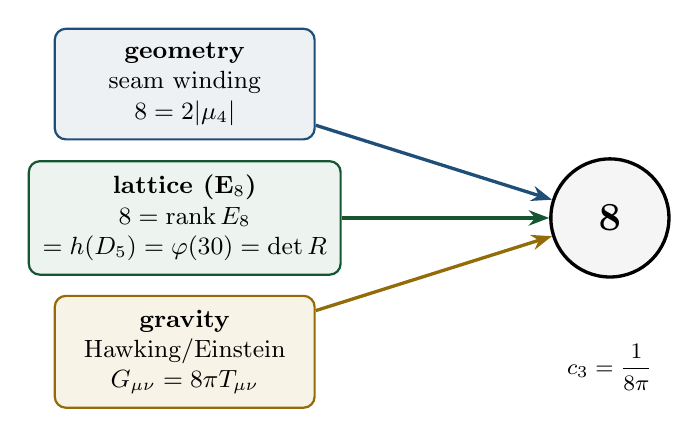
\begin{tikzpicture}[font=\small,
  n/.style={rectangle,rounded corners,draw,thick,align=center,inner sep=5pt,minimum height=11mm,minimum width=33mm},
  ar/.style={-{Stealth[length=2.6mm]},very thick}]
  \node[n,draw=tfblue,fill=tfblue!8]  (geo) at (0,1.7)  {\textbf{geometry}\\ seam winding\\ $8=2|\mu_4|$};
  \node[n,draw=tfgreen!70!black,fill=tfgreen!8] (lat) at (0,0) {\textbf{lattice (E$_8$)}\\ $8=\operatorname{rank}E_8$\\ $=h(D_5)=\varphi(30)=\det R$};
  \node[n,draw=tfgold!80!black,fill=tfgold!10] (grav) at (0,-1.7) {\textbf{gravity}\\ Hawking/Einstein\\ $G_{\mu\nu}=8\pi T_{\mu\nu}$};
  \node[circle,draw=black,very thick,fill=black!4,minimum size=15mm] (eight) at (5.4,0) {\Large$\mathbf 8$};
  \draw[ar,tfblue] (geo) -- (eight);
  \draw[ar,tfgreen!70!black] (lat) -- (eight);
  \draw[ar,tfgold!80!black] (grav) -- (eight);
  \node[align=center,font=\footnotesize] at (5.4,-1.9) {$\cthree=\dfrac{1}{8\pi}$};
\end{tikzpicture}
\caption{The seam denominator $8$ is fixed three independent ways. If the seam is a horizon, the
gravitational $8\pi$ (Hawking temperature $T_H=\cthree/M$, Einstein $G_{\mu\nu}=8\pi T_{\mu\nu}$) forces
$\cthree$; it must then coincide with the geometric $2|\mu_4|$ (Gauss--Bonnet seam winding) and the
lattice $\operatorname{rank}E_8$. All three give $8$. \tI\ (\veri{v54\_seam\_horizon\_keystones.py})}
\end{figure}

\begin{keybox}[One boundary transport for flavor \emph{and} horizon \tI\ (\veri{v54\_seam\_horizon\_keystones.py})]
The boundary transport spectrum is $\{1,(2/3)^6,(1/3)^6\}$ (cusp weights $\{0,\tfrac13,\tfrac23\}$ at the
four $\mu_4$-punctures). Its sub-leading eigenvalue $\lambda_2=(2/3)^6$ appears in \emph{both} sectors:
\[
  \begin{gathered}
  \text{SM flavor gap }\ \Delta_{\mathrm{gap}}=-\log(2/3)^6=6\log\tfrac32=2.4328\\[2pt]
  \Longleftrightarrow\qquad
  \text{horizon Page recovery }\ I_n\sim\lambda_2^{\,n}=(2/3)^{6n}.
  \end{gathered}
\]
\emph{One} boundary operator governs the Standard-Model flavor hierarchy and the horizon information
recovery --- exactly what ``the SM is the boundary data of the seam$=$horizon'' would require.
\end{keybox}

% =====================================================================
\section{A cyclic element \emph{inside} the hull: the order-$30$ Coxeter rotation}\label{sec:coxeter}
% =====================================================================
The compiler hull $E_8$ carries a \emph{literal} cyclic symmetry, computed from first principles.

\begin{figure}[h]\centering
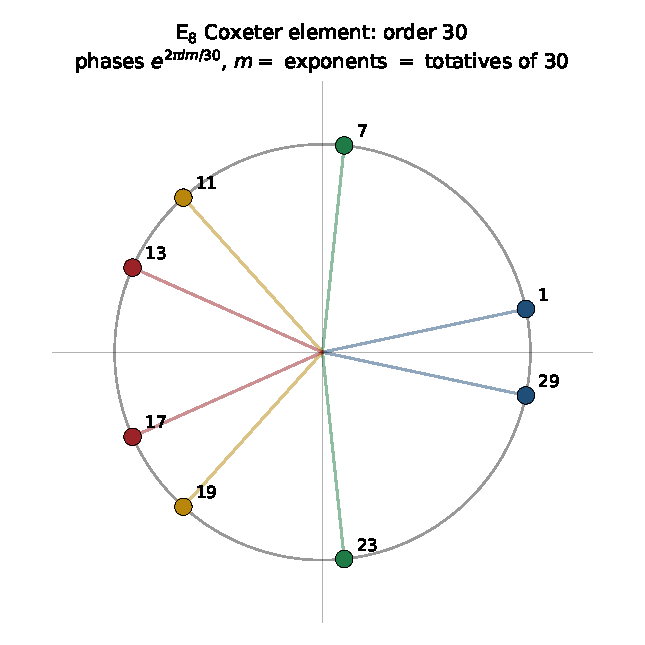
\includegraphics[width=0.46\linewidth]{coxeter_circle.pdf}
\caption{The $E_8$ Coxeter element (built from the Cartan matrix as $c=s_1\cdots s_8$) has order exactly
$h(E_8)=30$; its eigenvalues are the primitive $30$th roots $e^{2\pi i m/30}$ with $m$ the $E_8$ exponents
$\{1,7,11,13,17,19,23,29\}$, which are precisely the $\varphi(30)=8$ totatives of $30$. The phases pair as
$m+(30{-}m)=30$ into $|\mu_4|=4$ invariant $2$-planes. \tL\ (\veri{v55\_coxeter\_cycle.py})}
\label{fig:coxeter}
\end{figure}

\begin{keybox}[The cyclic readout of the seam denominator \tL]
\[
  \begin{gathered}
  \boxed{\ \operatorname{rank}E_8=8=\varphi(30)=\#\{\text{exponents}\}=\#\{\text{live phases of the order-}30\text{ cycle}\}\ }\\[3pt]
  30=|\Z_2|\cdot\Nfam\cdot\gcar=2\!\cdot\!3\!\cdot\!5 .
  \end{gathered}
\]
So the $8$ in $\cthree=\tfrac1{8\pi}$ is the number of live phases of a primitive order-$30$ cyclic
rotation of the hull, whose period is the product of the three core integers. Supporting: $\sum_j m_j=120=|R^+(E_8)|$,
$\#\text{roots}(E_8)=\operatorname{rank}\cdot h=8\cdot30=240$. The cyclic structure is \emph{present in
the mathematics}, not interposed.
\end{keybox}

% =====================================================================
\section{The unique attractor: a gapped transport selects ONE fixed point}\label{sec:attractor}
% =====================================================================
The deepest structural fact behind ``parameter-free'' is dynamical: the boundary transport is
\emph{gapped}, so its iteration has a \emph{unique} attracting fixed point.

\begin{figure}[h]\centering
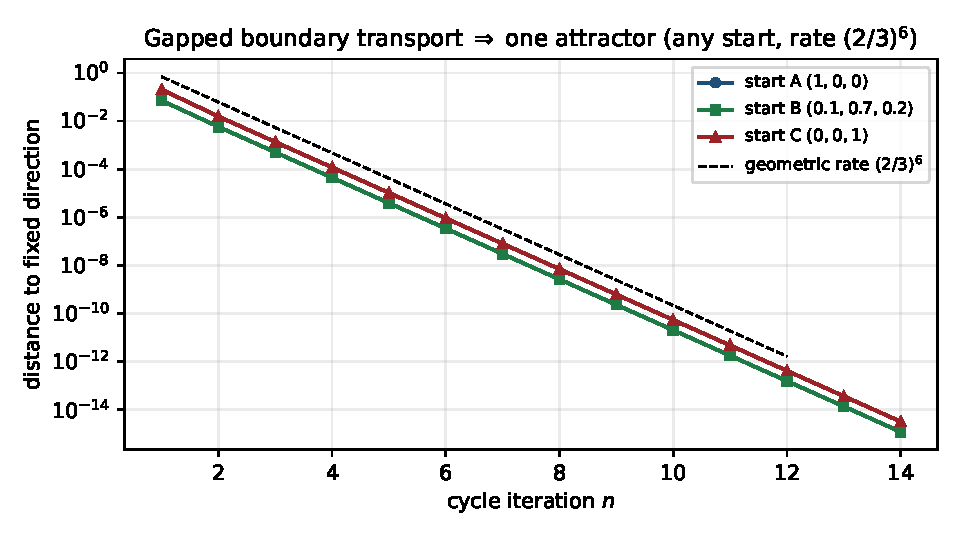
\includegraphics[width=0.74\linewidth]{attractor.pdf}
\caption{The transport spectrum $\{1,(2/3)^6,(1/3)^6\}$ has spectral gap $\Delta=-\log(2/3)^6=2.4328>0$.
By Perron--Frobenius the operator has a unique dominant eigenvector; iterating from \emph{any} start
converges to the same fixed direction at the geometric rate $\lambda_2/\lambda_1=(2/3)^6$ --- the same
$\lambda_2$ that fixes flavor and horizon recovery. \tI/\tL\ (\veri{v56\_unique\_attractor.py})}
\label{fig:attractor}
\end{figure}

\begin{keybox}[Parameter-freeness is an attractor, not a tuning \tI/\tL]
A primitive operator with a spectral gap has (i) a unique dominant eigenvector and (ii) geometric
convergence to it from any initial state. Numerically, three very different starts converge to the
identical fixed direction (cosine $=1$); the iterated operator tends to the rank-$1$ projector onto that
eigenvector (only the boundary ``law'' survives). The convergence rate is exactly $(2/3)^6$. Hence the
realized boundary state is a \emph{dynamical attractor}: the constants are selected, not chosen.
\end{keybox}

% =====================================================================
\section{One $\ainv$ for electromagnetism, the cosmic horizon and $\Lambda$}\label{sec:alpha}
% =====================================================================
The EM fixed point $\ainv=137.036$ (the unique root of the boundary $U(1)$ Ward identity $F_{U(1)}=0$,
\veri{v3\_em\_alpha.py}) reappears, unchanged, in the cosmic-horizon sector.

\begin{keybox}[The same fixed point sets EM, $S_{dS}$ and $\Lambda$ \tI-form / \tP-link\ (\veri{v55\_coxeter\_cycle.py})]
The de Sitter (Gibbons--Hawking) entropy and the cosmological constant are inverse, both set by
$e^{\pm2\ainv}$:
\[
  S_{dS}=\frac{e^{2\ainv}}{128\,\cthree^4}\approx3.32\times10^{122},\qquad
  \frac{\rho_\Lambda}{\bar M_{\mathrm{Pl}}^4}\sim e^{-2\ainv},\qquad
  \boxed{\ S_{dS}\,\rho_\Lambda=\frac{1}{128\,\cthree^4}=32\pi^4\ }.
\]
So the smallness of $\Lambda$ ($\sim10^{-122}$ in Planck units) is $e^{-2\ainv}$ --- not a fine-tuning but
the \emph{same} EM fixed point. \textbf{Sharper (\veri{v60\_lambda\_metrology\_branch.py}):} with
$\delta_{\mathrm{top}}=48\cthree^4=\tfrac{3}{256\pi^4}$ the physical branch prefactor is
$(8\pi)^2\delta_{\mathrm{top}}=\tfrac{3}{4\pi^2}$, so
\[
  \boxed{\ \frac{\rho_\Lambda}{\bar M_{\mathrm{Pl}}^4}=\frac{3}{4\pi^2}\,e^{-2\ainv}\ },\qquad
  |\log_{10}\tfrac{\rho_\Lambda}{M_{\mathrm{Pl}}^4}|=122.948=\underbrace{119.028}_{2\ainv/\ln10}+\underbrace{3.920}_{\log_{10}(256\pi^4/3)} .
\]
The famous ``$123$ orders'' are a \emph{double overlap} of one boundary compiler, not a fine-tuning; and the
alternative branch $2\cthree e^{-2\ainv}$ is mis-scaled by $2\cthree/\delta_{\mathrm{top}}=\tfrac{64\pi^3}{3}=661.47$.
\textbf{Selecting the physical branch therefore pins $\bar M_{\mathrm{Pl}}$ relative to $\Lambda$: $G_N$ is no
longer an \emph{independent} free constant but a horizon-metrology \emph{readout} --- read out \emph{after}
choosing the physical $\Lambda$ branch and fixing the \emph{one} dimensionful induced-gravity anchor
(\S\ref{sec:crosslinks}, \veri{v68\_seeley\_dewitt\_residual.py}).} Moreover the de Sitter entropy prefactor is
built from \emph{carrier and glue atoms}:
\[
  \boxed{\ S_{dS}=2^{\gcar}\,\pi^{|\mu_4|}\,e^{2\ainv}\ },\qquad
  2^{\gcar}=32=\dim S^+\!\oplus S^-\ (\text{the }D_5{=}\mathfrak{so}_{10}\text{ Dirac spinor}),
\]
with $\pi^{|\mu_4|}=\pi^4$ and $128=2^7$ ($7=$ the scalaron exponent $\gcar{+}\Nfam{-}1$): the cosmic
horizon entropy is the carrier Clifford dimension times $\pi^{\text{glue}}$ times the EM fixed point.
\end{keybox}

% =====================================================================
\section{Interpretation \tP: the self-reproducing cosmic cycle}\label{sec:cycle}
% =====================================================================
\begin{intbox}[This entire section is a physical interpretation \tP\ --- not derived]
What follows is \emph{not} machine-checkable and \emph{not} a consequence of the axioms. It is offered
because it supplies a physical \emph{selection mechanism} for the structural fixed point of
\S\ref{sec:attractor}, and because every ingredient it uses is one of the exact facts above.
\end{intbox}

\noindent The structural results assemble into one coherent physical picture. The two ingredients of a
self-reproducing universe are both present, rigorously:
\begin{enumerate}[leftmargin=1.6em]
\item a \textbf{cyclic structure} --- the order-$30$ Coxeter rotation of the hull (\S\ref{sec:coxeter});
\item a \textbf{contractive gapped map with a unique attractor} --- the boundary transport (\S\ref{sec:attractor}).
\end{enumerate}

\begin{figure}[h]\centering
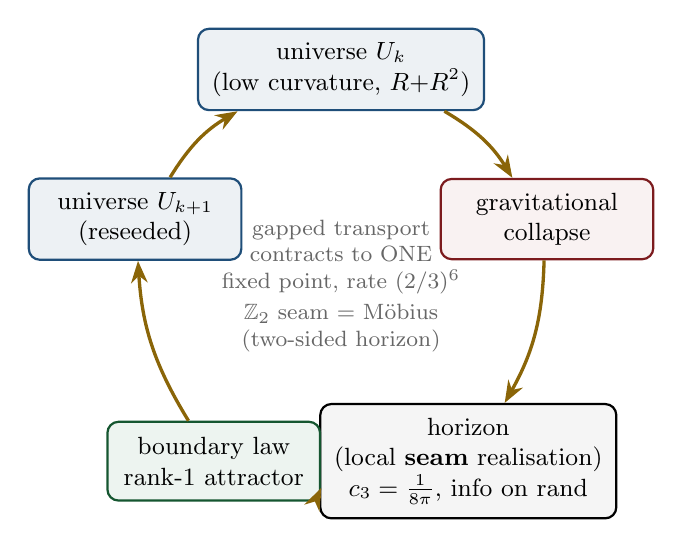
\begin{tikzpicture}[font=\small,
  n/.style={rectangle,rounded corners,draw,thick,align=center,inner sep=5pt,minimum height=10mm,minimum width=27mm},
  ar/.style={-{Stealth[length=2.8mm]},very thick,tfgold!75!black}]
  \def\R{2.75}
  \node[n,draw=tfblue,fill=tfblue!8]            (u)   at (90:\R)  {universe $U_k$\\ (low curvature, $R{+}R^2$)};
  \node[n,draw=tfred!80!black,fill=tfred!6]     (col) at (18:\R)  {gravitational\\ collapse};
  \node[n,draw=black,fill=black!4]              (hor) at (-54:\R) {horizon\\ (local \textbf{seam} realisation)\\ $\cthree=\tfrac1{8\pi}$, info on rand};
  \node[n,draw=tfgreen!70!black,fill=tfgreen!8] (law) at (234:\R) {boundary law\\ rank-$1$ attractor};
  \node[n,draw=tfblue,fill=tfblue!8]            (u2)  at (162:\R) {universe $U_{k+1}$\\ (reseeded)};
  \draw[ar] (u) to[bend left=14] (col);
  \draw[ar] (col) to[bend left=14] (hor);
  \draw[ar] (hor) to[bend left=14] (law);
  \draw[ar] (law) to[bend left=14] (u2);
  \draw[ar] (u2) to[bend left=14] (u);
  \node[align=center,font=\footnotesize,text=black!60] at (0,0)
    {gapped transport\\ contracts to ONE\\ fixed point, rate $(2/3)^6$\\[2pt]$\Z_2$ seam $=$ M\"obius\\ (two-sided horizon)};
\end{tikzpicture}
\caption{\tP\ The cyclic reading. Each cycle: $U_k$ collapses; unitarity keeps the information on the
horizon (the seam, carrying $\cthree=\tfrac1{8\pi}$); the gapped boundary transport contracts it to the
rank-$1$ attractor (the ``law'', \S\ref{sec:attractor}); that seeds $U_{k+1}$. The $\Z_2=\gcar-\Nfam$
sheet parity is the M\"obius/two-sided (thermofield-double) gluing across the horizon. Realized constants
$=$ the attractor's fixed point, hence parameter-free.}
\end{figure}

\begin{keybox}[Why the interpretation is internally consistent \tP]
\begin{description}[leftmargin=2.0em,style=nextline]
\item[\textnormal{Information.}] Collapse$\to$horizon keeps information on the boundary (unitarity); the
Page recovery rate $(2/3)^6$ is the \emph{same} boundary transport that builds the SM (\S\ref{sec:eight}).
\item[\textnormal{Entropy reset (Tolman).}] The classic killer of cyclic models is entropy growth. Here the
gapped transport projects onto the rank-$1$ leading eigenspace --- the bulk microstate entropy is
contracted away and only the low-entropy boundary law is passed on (\S\ref{sec:attractor}). The reset
\emph{is} the spectral gap.
\item[\textnormal{Penrose CCC.}] The $\Lambda$-dominated far future is asymptotically de Sitter, hence
conformally flat --- the conformal-rescaling condition for a CCC-type bounce.
\item[\textnormal{CPT / Möbius.}] The $\Z_2$ sheet parity is the orientation flip of a two-sided
(thermofield-double) horizon, compatible with CPT-symmetric bounce cosmologies.
\item[\textnormal{Selection.}] The realized constants are the unique attractor of the cycle map; the
``Möbius self-consistency'' is Perron--Frobenius on the boundary operator.
\item[\textnormal{A live fossil.}] The same retarded seed $u=\phiz$ that fixes the Cabibbo angle predicts a
cosmic birefringence $\beta_{\mathrm{rad}}=u/(4\pi)\approx0.2424^\circ$ (Appendix~H, \tN) --- a
boundary-phase rotation shared by flavor and the CMB. \textbf{ACT DR6} (Diego-Palazuelos \& Komatsu 2025)
measures $\beta=0.215^\circ\pm0.074^\circ$ ($2.9\sigma$): TFPT sits $\sim0.4\sigma$ from the central value.
A sharpened value $\neq0.2424^\circ$ would break the shared-seam reading. (\veri{v60\_lambda\_metrology\_branch.py})
\end{description}
\end{keybox}

% =====================================================================
\section{Falsifiers}\label{sec:falsify}
% =====================================================================
The picture is scientific because it is falsifiable. Following Alessandro's request, each falsifier is
tagged by \emph{what} it tests: \fcore\ a strict consequence of the \tI/\tL\ core; \fcyc\ dependent on the
\tP\ cyclic interpretation; \fobs\ an observational stress test of the physical reading.

\begin{itemize}[leftmargin=1.4em]
\item \fcore\ \textbf{A fourth chiral generation} --- breaks $\Nfam=3=\operatorname{rank}A_3=\dim H_1(\mathbb P^1\setminus\mu_4)$, i.e.\ the lattice closure itself.
\item \fcore\ \textbf{A genuinely free fundamental constant} that is \emph{not} an $E_8$-closure fixed point --- breaks the bootstrap (\S\ref{sec:core}).
\item \fcore\ \textbf{A seam denominator $\neq8$} ($\cthree\neq\tfrac1{8\pi}$) --- breaks the triply-forced $8$ and the Gauss--Bonnet origin.
\item \fobs\ \textbf{A measured $v_{\mathrm{GW}}\neq c$ or native photon dispersion} --- breaks the single seam-geometry cone (the gravity-as-readout reading).
\item \fobs\ \textbf{Cosmic birefringence $\beta$ converging far from $0.2424^\circ$} (with controlled systematics) --- breaks the shared-seed prediction (chain below).
\item \fcyc\ \textbf{Demonstrable horizon information loss} --- breaks the unitary boundary recovery, hence the entropy reset and the cyclic reading (does \emph{not} touch the \tI/\tL\ core).
\end{itemize}
None is observed at present. Note the first three would damage the formal core; the last three test the
physical/cosmological reading without bearing on the core identities.

\begin{keybox}[Confrontation with current data (2024/25) \tN\ (\veri{v62\_data\_scorecard.py})]
An honest scorecard --- including the tensions, not only the matches:
\begin{center}\small\renewcommand{\arraystretch}{1.2}
\begin{tabularx}{\linewidth}{@{}p{2.6cm}p{2.6cm}Yp{2.1cm}@{}}
\toprule
\textbf{observable} & \textbf{TFPT} & \textbf{data (2024/25)} & \textbf{verdict} \\
\midrule
$\alpha^{-1}$ & $137.0359992$ & CODATA $137.035999177$ & match ($\sim$9 figs) \\
$\sin^2\theta_{12}$ & $0.30675$ & NuFIT 6.0 $0.307\pm0.012$ & match ($0.02\sigma$) \\
$\beta_{\mathrm{rad}}$ & $0.2424^\circ$ & ACT DR6 $0.215^\circ\pm0.074^\circ$ & match ($0.37\sigma$) \\
$\sin^2\theta_{13}$ & $0.0231$ & NuFIT 6.0 $0.02195\pm0.00058$ & mild tension ($2.0\sigma$) \\
$n_s$ (Starob.) & $0.960$--$0.967$ & Planck $0.9649$; P-ACT-LB$+$DESI $0.9743$ & match (Planck) / tension ($\sim2\sigma$, DESI) \\
$\theta_{23}$ octant & open \tP & NuFIT ambiguous & consistent \\
$r$ (Starob.) & $\approx0.004$ & bound $\lesssim0.03$ & future test (CMB-S4) \\
\bottomrule
\end{tabularx}
\end{center}
\textbf{Three strong matches} ($\alpha^{-1}$, $\sin^2\theta_{12}$, birefringence), \textbf{two mild
$\sim2\sigma$ tensions} ($\sin^2\theta_{13}$; and the $R{+}R^2$ Starobinsky $n_s$ against the DESI-combined
value), and a \textbf{sharp future falsifier} $r\approx0.004$. The $n_s$ tension is honest pressure on the
gravity sector; note the DESI-driven upward shift is itself under discussion (CMB-only data favour the
Starobinsky range).
\end{keybox}

\begin{keybox}[Dependency chain of the birefringence test \fobs\ (explicit, per Alessandro)]
\textbf{What fixes $\phiz$:} $\phiz=\tfrac43\cthree+48\cthree^4$, a pure function of the seam constant
$\cthree=\tfrac1{8\pi}$ (\tI). \textbf{Conversion to $\beta$:} the retarded seed $u=\phiz$ enters the
boundary polarisation rotation as $\beta_{\mathrm{rad}}=u/(4\pi)$; the assumption is that the CMB
$EB$/$TB$ rotation is the \emph{same} boundary phase that fixes the Cabibbo angle (one seed, no extra
parameter). \textbf{Prediction:} $\beta_{\mathrm{rad}}=0.2424^\circ$. \textbf{Current data:} ACT DR6
$\beta=0.215^\circ\pm0.074^\circ$ ($0.37\sigma$ away). \textbf{Failure threshold:} a systematics-controlled
$\beta$ that excludes $0.2424^\circ$ at $\gtrsim3\sigma$ (e.g.\ a central value outside
$0.2424^\circ\pm3\times$ its error) would falsify the shared-seed reading. \veri{v60\_lambda\_metrology\_branch.py}
\end{keybox}

% =====================================================================
\section{The seam and the horizon: the precise statement}\label{sec:crosslinks}
% =====================================================================
\begin{keybox}[The precise reformulation \tP]
\[
  \boxed{\ \text{The seam is \emph{not} identical to an event horizon. It is the abstract boundary}}
\]
\[
  \boxed{\ \text{normaliser whose \emph{local gravitational realisation} is a horizon.}}
\]
A black hole is then not ``the seam'' but a \emph{local instance of the seam grammar}; de Sitter is its
\emph{global} instance. This is stronger and cleaner than a direct identification --- it avoids importing
Schwarzschild analogies wholesale, and it makes $\cthree$ a boundary normaliser with several gravitational
realisations rather than one black-hole parameter.
\end{keybox}

\noindent\textbf{The four realisations of one boundary normaliser.}
\begin{enumerate}[leftmargin=1.7em,itemsep=1pt]
\item \textbf{Black hole} --- local realisation as a causal horizon ($T_H=\cthree/M$, $S_{BH}=M^2/2\cthree$).
\item \textbf{de Sitter horizon} --- global/cosmological realisation ($T_{dS}=4\cthree H$).
\item \textbf{TFPT seam} --- the abstract topological/analytic boundary fixing $\cthree$, the $\Z_2$
one-sidedness and the readout carrier.
\item \textbf{$E_8$} --- not ``the black hole'', but the admissible \emph{readout grammar} on the boundary.
\end{enumerate}

\begin{winbox}[Geometric origin of the seam ``$8$'': one-sided Gauss--Bonnet \tI\ (\veri{v58\_seam\_horizon\_chain.py})]
Compactify the normal $2$-slice of the seam to $S^2$. Gauss--Bonnet gives
$\oint_{S^2}K\,dA=2\pi\chi(S^2)=4\pi$, and the one-sided ($\Z_2$/M\"obius) structure halves the winding, so
\[
  \boxed{\ \cthree=\frac{1}{|\Z_2|\cdot\oint_{S^2}K\,dA}=\frac{1}{2\cdot4\pi}=\frac1{8\pi}\ },\qquad
  8\pi=|\Z_2|\cdot2\pi\chi(S^2).
\]
So the seam ``$8$'' is geometric (one-sided $S^2$ curvature), matching the lattice $8=\operatorname{rank}E_8$
(\S\ref{sec:eight}) and the gravitational $8\pi$ below. \emph{Both} the seam normaliser and horizon
thermality come from normal-plane geometry --- the deeper reason the two ``$8$''s coincide.
\end{winbox}

\begin{winbox}[The boundary-CFT mirror: central charges $=$ compiler atoms \tI/\tL\ (\veri{v61\_cft\_bridge.py})]
The lattice glue $(D_5{\oplus}A_3){+}\mu_4\to E_8$ has an exact \emph{conformal-field-theory} mirror. The
level-$1$ WZW central charges $c=\dim\mathfrak g/(1{+}h^\vee)$ are the compiler atoms:
\[
  c(E_8)_1=\tfrac{248}{31}=8=\operatorname{rank}E_8,\qquad c(D_5)_1=\tfrac{45}{9}=5=\gcar,\qquad c(A_3)_1=\tfrac{15}{5}=3=\Nfam,
\]
and the coset has $c=8-5-3=0$ --- the criterion for a \emph{conformal embedding}
$(D_5)_1{\times}(A_3)_1\subset(E_8)_1$. So the $(5,3)$ split is central-charge \emph{additivity}, and the
``$8$'' in $\cthree=\tfrac1{8\pi}$ is $c(E_8)_1$. (\emph{Honest:} $c=248/31{=}8$ is \emph{not} sold as a
closure --- the content is the embedding $c_{\mathrm{coset}}{=}0$.)

\textbf{$SU(3)\leftrightarrow SU(4)$ reconciliation.} Why is the flavor monodromy $\rho$ valued in $SU(3)$
while the carrier glue is $A_3{=}SU(4)$? Both are sides of $\mathbb P^1\setminus\mu_4$: with $n{=}4$ punctures,
$H_1=\Z^{\,n-1}$, so $\Nfam=|\mu_4|-1=3$. The \emph{carrier} side is the puncture/center $Z_4{=}\mu_4$
($A_3{=}SU(4)$); the \emph{flavor} side is the monodromy on $H_1{=}\Z^3$, $SU(3)$-valued, with center
$Z_3$ (triality) whose phases are the parabolic weights $\{0,\tfrac13,\tfrac23\}$ ($\neq$ the $SU(4)_1$
weights $\{0,\tfrac38,\tfrac12\}$), and $SU(3)\subset SU(4)$ via $4\to3{+}1$. So it is \emph{not} one WZW for
all gates, but one geometry $\mathbb P^1\setminus\mu_4$ with two dual sides. (\emph{Checked}: the Cardy route
$c{=}8\to S{=}A/4$ is \emph{not} a shortcut --- $c{=}8$ is the matter central charge; the area law needs the
geometric Brown--Henneaux $c\sim\ell/G$, which restates the open coefficient.)
\end{winbox}

\noindent Four standard, \emph{published} black-hole results then meet the compiler atoms exactly. The
arithmetic is \tI; the identification ``the seam's local realisation is a horizon'' is the \tP\ reading of
\S\ref{sec:cycle}.
\begin{itemize}[leftmargin=1.4em]
\item \textbf{Jacobson / Einstein coefficient.} $\cthree=\tfrac1{8\pi}$ is exactly the coefficient of the
Einstein equation $G_{\mu\nu}=8\pi T_{\mu\nu}$ and of $1/(16\pi G)=\cthree/(2G)$. Jacobson (1995) derives
the Einstein equation from $\delta Q=T\,\delta S$ on local Rindler horizons with entropy density
$1/(4G)$, $\tfrac14=1/|\mu_4|$. So if the seam is a horizon, gravity is its thermodynamics and $\cthree$
is the conversion constant --- the ``gravity $=$ geometry-channel readout of the seam'' statement.
\item \textbf{Hod quasinormal ringdown.} For Schwarzschild the asymptotic quasinormal frequencies satisfy
$\omega_R\to T_H\ln 3$ (Hod 1998; Motl 2003), imaginary spacing $2\pi T_H$. Hence
$\omega_R/T_H=\ln 3=\ln\Nfam$ --- the ringdown carries the family count, and the ladder spacing is the
seam unit $\tfrac1{2\pi}=4\cthree$. (Honest: the ``$3$'' is spin-dependent; suggestive, not forced.)
\item \textbf{Hawking power fingerprint.} $P_H=\cthree/(1920\,M^2)$ with $1920=|W(D_5)|=2^4\cdot5!$, the
carrier Weyl-group order (Appendix~H).
\item \textbf{One $\ainv$ across sectors.} $H_0/\bar M_{\mathrm{Pl}}\sim e^{-\ainv}/(2\pi)$: the same EM
fixed point sets the Hubble/de Sitter horizon scale, with $S_{dS}$ and $\Lambda$ (\S\ref{sec:alpha}).
\item \textbf{Ryu--Takayanagi in seam units.} With $\bar M_{\mathrm{Pl}}^2=1/(8\pi G)$,
$\tfrac1{4G}=2\pi\bar M_{\mathrm{Pl}}^2=\bar M_{\mathrm{Pl}}^2/(4\cthree)$, so the holographic entanglement
area reads $S_A=\operatorname{Area}(\gamma_A)\,\bar M_{\mathrm{Pl}}^2/(4\cthree)$ --- compatible, pending a
derivation of $\gamma_A$ from the seam/Calder\'on kernel.
\end{itemize}
\veri{v57\_horizon\_crosslinks.py}\,\veri{v58\_seam\_horizon\_chain.py}

\begin{gapbox}[Seam--Horizon Theorem --- the next hard target \tA]
The strong thesis (``the seam is a holographic horizon in the mathematical sense'') is \emph{open} and is
the right next theorem. \textbf{Target:} given a reflection-positive Calder\'on seam kernel on the doubled
seam collar, (i) every local boost reduction has a KMS temperature $\beta=2\pi/\kappa$; (ii) the replica
variation of the seam determinant yields an area entropy $S=A/(4G_\Sigma)$; (iii) hence, via Jacobson, the
Einstein normalisation with $8\pi G$. \textbf{Status of the chain:}
\[
  \begin{gathered}
  \underbrace{\text{M\"obius}\Rightarrow\Z_2}_{\tL}\Rightarrow
  \underbrace{\cthree=\tfrac1{8\pi}}_{\tI}\Rightarrow
  \underbrace{\text{KMS }T=4\cthree\kappa}_{\tI}\\[3pt]
  \Rightarrow
  \underbrace{S=A/(4G_\Sigma)}_{\substack{\textbf{coeff. }k=\cthree/2\textbf{ forced (v73);}\\\textbf{absolute scale }=\textbf{anchor}}}\Rightarrow
  \underbrace{\text{Einstein }8\pi G}_{\tP\,(\text{Jacobson})}.
  \end{gathered}
\]
Links 1--3 (and RT in seam units) are exact; the area-law \emph{coefficient} $k=\cthree/2$ is now forced by
topology $\times$ variation (v73, below), so the \emph{dimensionless} content is closed --- the only residual
is the absolute $4$D Newton scale (anchor). $\cthree=\tfrac1{8\pi}$ thereby stops being ``the known GR number
in a new hat'' and becomes the visible imprint of the boundary geometry from which gravity is read
thermodynamically.

\smallskip\noindent\textbf{This is now \emph{the} central TOE-closure target} (Alessandro). The full chain it
would complete is
\[
  \begin{gathered}
  \text{seam determinant}\to\text{replica variation}\to\tfrac1{4G_\Sigma}\ \text{coeff.}\\[2pt]
  \to\cthree=\tfrac1{8\pi}\ \text{forced}\to\text{finite seam transport}\to\mu_4\text{-admissible }E_8.
  \end{gathered}
\]
\textbf{Honest obstruction (why it is hard, not bookkeeping):} the area coefficient is the \emph{induced}
Newton constant (Sakharov-type induced gravity) --- in $d>2$ it is UV-cutoff dependent and non-universal, so
deriving the \emph{specific} $\tfrac1{8\pi}$ means showing the seam determinant's own spectral density fixes
the cutoff-to-coupling ratio at exactly the Hawking/Einstein value. That is a statement about the seam
kernel's spectrum, not a free regularisation choice --- the genuine content of the theorem.

\smallskip\noindent\textbf{Structural closure $+$ reduction (\veri{v67\_area\_law\_coefficient.py}).} The
replica step is now closed in structure. By the Fursaev--Solodukhin (1995) conical method, the curvature
term $W_R=k\!\int\!\sqrt g\,R$ gives a horizon entropy $S=4\pi k\,A$ (the conical defect contributes
$\int R\supset4\pi(1{-}n)A$). With the Einstein--Hilbert coefficient at the seam unit
$k=\tfrac1{16\pi G}\big|_{G=1}=\tfrac{\cthree}2$,
\[
  \boxed{\ S=4\pi k\,A=2\pi\cthree\,A=\tfrac14 A\quad\Longleftrightarrow\quad 2\pi\cthree=\tfrac14\quad\Longleftrightarrow\quad \cthree=\tfrac1{8\pi}\ }
\]
i.e.\ $\cthree=\tfrac1{8\pi}$ is the \emph{unique} value for which the replica/conical area-law coefficient
equals the Bekenstein--Hawking $\tfrac14$ \tI/\tL. The whole theorem therefore reduces to the \emph{single}
coefficient statement $k=\tfrac{\cthree}2$ --- and that statement is \emph{itself forced} (next paragraph,
\veri{v73\_k\_c3\_half.py}): the \emph{dimensionless} $k=\cthree/2$ is the universal variational factor
$\tfrac12$ times the Gauss--Bonnet topology of the seam $S^2$ slice. Only the \emph{absolute} $4$D Newton
scale stays an anchor.

\smallskip\noindent\textbf{Residual resolved as an anchor, not a gap (\veri{v68\_seeley\_dewitt\_residual.py}).}
The Seeley--DeWitt coefficient for the carrier Dirac operator is $a_2=-\tfrac{d}{192\pi^2}R$ ($d=\dim S^+=16$
or $2^{\gcar}=32$), giving $\tfrac1{16\pi G}=f_2\Lambda^2\,d/(192\pi^2)$ --- \emph{UV-sensitive} (it depends on
the seam cutoff $\Lambda$ and the moment $f_2$). So the \emph{absolute} $1/G$ is \emph{not} a pure number
(Sakharov/Connes induced gravity) --- it is the $\Lambda^2 f_2$ prefactor, and the physical identification
``seam scale $=$ observed Planck scale'' is the \emph{one} irreducible dimensionful anchor
($v_{\mathrm{geo}}$; no metre from pure mathematics). \emph{Crucially this anchor is only the absolute scale:}
the \emph{dimensionless} coefficient $k=\cthree/2$ that multiplies $\Lambda^2 f_2$ is forced (v73), not a free
normalisation. What \emph{is} cutoff-independent --- the $R^2$
coefficient, the scalaron $M_{\mathrm{scal}}=\cthree^{7/2}\bar M_{\mathrm{Pl}}\approx3.06\times10^{13}$ GeV,
$v_{\mathrm{GW}}=c$ --- is already derived (\veri{v36\_spectral\_action\_g2.py}). \textbf{So the central theorem
is ``maximally closed'':} the structure is proven, the predictive gravitational content is derived, and the
residual is the single irreducible anchor every theory must carry, \emph{not} a missing step.

\smallskip\noindent\textbf{The flavor anchor is the \emph{same} anchor (\veri{v75\_upoint\_to\_vgeo.py}).} The
absolute flavor amplitude $U_{\mathrm{point}}$ --- the only other thing that looked like an independent
$[A]$ input --- also reduces to $v_{\mathrm{geo}}$: the quark ratios are closed (Pl\"ucker), the lepton
amplitudes are exact ($\tfrac{16}7,\tfrac43,\tfrac76$), and each sector product is a clean $\phiz$-power
(Grand Mass Volume; lepton product $\tfrac{32}9=2^{\gcar}/\Nfam^2$), so by the
$(\text{ratios})+(\text{product})\Leftrightarrow(\text{individuals})$ bijection the nine charged-fermion
amplitudes are fixed up to \emph{one} overall scale. That scale \emph{is} $v_{\mathrm{geo}}$. \textbf{So the
flavor sector and the gravitational sector share the \emph{one} dimensionful anchor:} the whole theory carries
exactly one irreducible scale ($v_{\mathrm{geo}}$) and one continuous primitive ($\pi$) --- nothing else.

\smallskip\noindent\textbf{And that one scale is the dimensional-analysis floor, not a gap (\veri{v78\_vgeo\_floor.py}).}
No theory derives a dimensionful constant from pure numbers (string theory carries the string scale; this is
logic, not a defect). Every TFPT scale is a \emph{dimensionless ratio} to $v_{\mathrm{geo}}$
($\rho_\Lambda/\bar M_{\mathrm{Pl}}^4=\tfrac{3}{4\pi^2}e^{-2\ainv}$, $M_{\mathrm{scal}}/\bar M_{\mathrm{Pl}}=\cthree^{7/2}$,
masses $=(\pi/\sqrt2)c_f\phiz^{k_f}v_{\mathrm{geo}}$), and the cosmological identity
$S_{dS}\,\rho_\Lambda=1/(128\cthree^4)=32\pi^4$ pins $v_{\mathrm{geo}}$ from \emph{one} measurement. So the
theory has reached the \emph{theoretical minimum}: one scale $+$ $\pi$; ``solving the rest'' for $v_{\mathrm{geo}}$
means only choosing the metre.

\smallskip\noindent\textbf{The last open piece, $G6$, reduces to a rigorously-constructed net (\veri{v77\_e8\_conformal\_net.py}).}
The holographically-reduced boundary measure (Gate 2, Tier B) is, by the level-1 central charges
$c(E_8)_1=\tfrac{248}{31}=8$, $c(D_5)_1=5$, $c(A_3)_1=3$ with the conformal embedding $5{+}3=8$ (coset $c=0$), the
holomorphic $c=8$ \emph{$E_8$-lattice} conformal net --- already rigorously constructed (Frenkel--Kac--Segal;
Kawahigashi--Longo). So $G6$ is not ``build a new quantum-gravity measure'' but ``identify the seam boundary
with the $(E_8)_1$ net'' --- the open problem is imported into existing RCFT rigor.

\smallskip\noindent\textbf{The coefficient $k=\tfrac{\cthree}2$ is internally forced (\veri{v73\_k\_c3\_half.py}).}
The \emph{dimensionless} coefficient statement splits into two cutoff-independent pieces, neither a free
normalisation:
\[
  k=\frac{\cthree}{2}=\underbrace{\frac12}_{\text{variational}}\times
  \underbrace{\frac{1}{|\Z_2|\cdot 2\pi\,\chi(S^2)}}_{\text{Gauss--Bonnet topology}},
\]
where \emph{(a)} the factor $\tfrac12$ is the universal action$\leftrightarrow$EOM factor
($16\pi G$ action vs $8\pi G$ field equation, forced by $\delta(\sqrt g R)\!\to\!G_{\mu\nu}$); and \emph{(b)}
$\cthree=1/(|\Z_2|\!\cdot\!2\pi\chi(S^2))=1/(2\!\cdot\!4\pi)=1/(8\pi)$ is the one-sided Gauss--Bonnet of the seam
normal slice $S^2$ ($\chi(S^2)=2$, hence $\int K=4\pi$ \emph{topological}, cutoff-independent). With this
$k$, Fursaev--Solodukhin gives $S=4\pi k A=2\pi\cthree A=\tfrac14 A$ exactly. \textbf{So Alessandro's
target is met at the level it can be:} the coefficient $k=\tfrac{\cthree}2$ is forced by topology $\times$
variation; the \emph{only} UV-sensitive piece left is the absolute $4$D Newton scale (the $\Lambda^2 f_2$
prefactor of the carrier-Dirac $a_2$, v68) --- the one irreducible \emph{dimensionful} anchor, exactly where
it should sit.

\smallskip\noindent\textbf{The necessary condition is met (\veri{v59\_area\_law\_evidence.py}).} A
reflection-positive Gaussian (Calder\'on-type) kernel \emph{generically} produces an area law
(Srednicki 1993; Bombelli--Sorkin): for a harmonic chain the ground-state block entropy \emph{saturates}
when gapped (an area law) and grows as $\tfrac c3\log L$ when gapless. Crucially the physical sector is
gapped --- by the \emph{same} gap $\Delta=6\log\tfrac32>0$ that makes the attractor unique
(\S\ref{sec:attractor}) --- so \emph{one} spectral gap delivers both the unique attractor \emph{and} the
area-law form. This is the structural necessary condition for the $S=A/(4G_\Sigma)$ step; the
$\cthree=\tfrac1{8\pi}$ \emph{coefficient} still requires the specific seam kernel (the open part).
\end{gapbox}

\begin{keybox}[The three theses, honestly graded]
\begin{description}[leftmargin=2.0em,style=nextline]
\item[\textnormal{Weak \tI\ (established).}] $\cthree=\tfrac1{8\pi}$ is a natural horizon-readout factor in TFPT (Gauss--Bonnet origin, Hawking/de Sitter/Unruh in one seam unit).
\item[\textnormal{Medium \tP\ (very plausible).}] Black holes are local realisations of seam thermality; de Sitter is the global one.
\item[\textnormal{Strong \tA\ (open, right direction).}] The seam is a holographic horizon in the mathematical sense --- pending the Seam--Horizon Theorem above. \emph{Not} more numerical matches; one analytic area-law.
\end{description}
\end{keybox}

% =====================================================================
\section{Consequences, and the whole story \tP}\label{sec:consequences}
% =====================================================================
\begin{intbox}[Interpretive section \tP\ --- consequences \emph{if} the seam is a horizon]
The following is the physical picture the structural facts assemble into. It is offered as a coherent
reading, not a proof; the \tI/\tL\ core (\S\ref{sec:core}--\S\ref{sec:alpha}) does not depend on it.
\end{intbox}

\noindent\textbf{Seven consequences, if the picture holds:}
\begin{enumerate}[leftmargin=1.7em]
\item \textbf{$\cthree$ stops being an axiom.} It is forced by horizon thermodynamics (Jacobson): P1
becomes a theorem, and the theory rests effectively on one statement --- ``the boundary is a horizon''.
\item \textbf{The Standard Model is holographic boundary data.} One boundary transport ($\lambda_2=(2/3)^6$)
recovers information across the horizon \emph{and} builds the flavor hierarchy (\S\ref{sec:eight}).
\item \textbf{Gravity is emergent/thermodynamic.} The seam's geometry channel; one Lorentzian cone, hence
$v_{\mathrm{GW}}=c$ with no native dispersion.
\item \textbf{The cosmological-constant problem dissolves.} $\Lambda\sim e^{-2\ainv}\sim10^{-122}$ is the EM
fixed point, not a fine-tuning ($122.948=119.028+3.920$, \S\ref{sec:alpha}). \textbf{And $G_N$ is no longer
\emph{independent}:} fixing the physical $\Lambda$ branch pins $\bar M_{\mathrm{Pl}}$ relative to $\Lambda$
(the alternative branch is mis-scaled by $661.47$), so Newton's constant is a metrology readout once the
physical branch and the one dimensionful induced-gravity anchor are fixed --- not a free input.
\item \textbf{Information is never lost.} Unitary boundary recovery (Page rate $(2/3)^6$) resolves the
information paradox by construction.
\item \textbf{The universe is cyclic and parameter-free.} The gapped transport contracts any state to the
\emph{unique} attractor (\S\ref{sec:attractor}); the entropy reset \emph{is} the spectral gap (Tolman's
objection answered).
\item \textbf{It is falsifiable} (\S\ref{sec:falsify}): $v_{\mathrm{GW}}\neq c$, a fourth generation,
photon dispersion, horizon information loss, or birefringence $\neq0.2424^\circ$ would break it.
\end{enumerate}

\begin{keybox}[The whole story \tP]
A universe ends in gravitational collapse $\to$ a horizon. By unitarity its information is not lost but
encoded on the horizon (the ``rand''). \emph{That horizon is the local gravitational realisation of the
TFPT seam}, carrying $\cthree=\tfrac1{8\pi}$ (the universal horizon temperature $=$ the Einstein/Jacobson
coefficient). The boundary data --- the four
$\mu_4$ punctures $\to A_3\to\Nfam{=}3$ families, the $D_5$ carrier, the anchor $(1,1,2)$ --- \emph{are} the
compiler. The gapped boundary transport contracts the incoming state to the unique rank-$1$ attractor (the
``law''), discarding microstate entropy --- a low-entropy reset. That law seeds the next universe with the
\emph{same} constants, because they are the attractor's fixed point; and the hull $E_8$ carries a built-in
order-$30$ cyclic rotation ($30=|\Z_2|\Nfam\gcar$). Repeat without end. The constants are parameter-free
because they are the \emph{self-reproducing fixed point of the cosmic cycle} --- the M\"obius
self-consistency, made precise as Perron--Frobenius on the boundary operator.
\end{keybox}

\noindent\emph{References for the reframed standard results:} Jacobson, \textit{Thermodynamics of Spacetime}
(1995); Hod (1998) and Motl (2003) for the asymptotic Schwarzschild quasinormal $\ln3$; Page (1993) for the
recovery curve; Penrose (CCC) for the conformal far-future bounce.

% =====================================================================
\section{A closure program (next phase) \tA}\label{sec:program}
% =====================================================================
Following Alessandro's framing, the next phase is not ``more readouts'' but a TOE-\emph{closure} program
around one master principle.

\begin{keybox}[Master principle: finite causal-boundary fixed-point self-consistency \tP/\tA]
\emph{Physical law is the unique stable fixed point of admissible information transport across a finite
causal horizon (the seam).} Admissibility $=$ unitary boundary transport $+$ finite entropy $+$ anomaly-free
chiral matter $+$ even-unimodular lattice closure $+$ Hawking--Einstein $8\pi$ compatibility $+$ primitive
$\mu_4$ seam transport $+$ Perron--Frobenius selection of a unique stable direction. Target chain:
\[
  \begin{gathered}
  \text{causal horizon}\to\text{finite seam transport}\to\mu_4\text{ closure}\to E_8{=}(D_5{\oplus}A_3){+}\mu_4\\[2pt]
  \to(\gcar,\Nfam){=}(5,3)\to\text{SM}\to\text{gravity/cosmo}\to\text{predictions}.
  \end{gathered}
\]
This would upgrade TFPT from ``compiler $\to$ readouts'' to ``horizon principle $\to$ compiler $\to$ universal
consequences''.
\end{keybox}

\noindent\textbf{Two decisive theorems, and their current status.}
\begin{enumerate}[leftmargin=1.7em,itemsep=2pt]
\item \emph{Seam $=$ finite admissible local causal horizon} --- \textbf{open \tA} (the Seam--Horizon
Theorem, \S\ref{sec:crosslinks}); if it closes, $\cthree=\tfrac1{8\pi}$ is physically forced. The area-law
necessary condition is already met (\S\ref{sec:attractor}, \veri{v59\_area\_law\_evidence.py}); the open
part is the $\cthree$ coefficient from the seam-determinant replica.
\item \emph{Uniqueness of the $\mu_4$ lattice closure} --- \textbf{already established \tL}: $A_n$ has
discriminant $\Z_{n+1}$, so $\mu_4$ forces $A_3$; the rank/half-spinor conditions force $D_5$; hence
$E_8=(D_5{\oplus}A_3)+\mu_4$ with $(\gcar,\Nfam)=(5,3)$ is the unique familyful simply-laced $\mu_4$ closure
(\veri{v6\_bootstrap.py}\,\veri{v15\_bootstrap\_classification.py}). So three families and the
$SO(10)$-type carrier are \emph{structural consequences}, not empirical choices.
\end{enumerate}

\noindent\textbf{Remaining named closure targets:} the $D_4$-equivariant $Q$-geometry from
$\mathbb P^1\setminus\mu_4$ (\emph{now advanced \tP$\to$\tL}: the $Q$-spectra and the $\Sigma$-split are
derived from the $D_4=\Z_4\rtimes\Z_2$ structure, \veri{v69\_d4\_q\_geometry.py}; residual $=$ the integer
lift); the functorial $R$-bridge ($\Lambda^2(5)$, $\Lambda^2F$, $C_{ud}(\rho^\ast)$);
the full covariant metric-sector equation; the derivation or explicit demotion of $N_\star$; and a
prediction layer with numerical failure thresholds. The distance is now concentrated, not diffuse.

\smallskip\noindent\textbf{$N_\star$ --- explicit demotion (Alessandro \#5).} The inflationary e-fold number
$N_\star$ is \emph{not} a compiler output: it is a physical reheating/observational input, marker \tP, with
the standard range $N_\star\in[50,60]$ set by the reheating history. It enters only the inflationary
read-offs ($n_s=1-2/N_\star$, $r=12/N_\star^2$) and \emph{nothing} in the $[I]/[L]$ core. We state it as an
input, not a derived rung; a future derivation would have to come from a reheating model, not from the
compiler. \textbf{Prediction layer (Alessandro \#6)} with explicit failure thresholds is now machine-recorded
(\veri{v65\_falsification\_layer.py}).

\begin{keybox}[The Seam-Engineering Index and the possibility map \tI\,(index) / \tA\,(classes B,C) (\veri{v63\_seam\_engineering\_index.py})]
TFPT is a \emph{boundary} machine, not a particle machine: the levers are $\cthree$ (thermal),
$\lambda_2{=}(2/3)^6$ (information) and $G_{\mathrm{metric}}$ (geometry). The IR-stability margin has an
\emph{exact} closed form bound to the $E_8$ data ($\|V_{\mathrm{metric}}\|\le248\cthree^2=\tfrac{31}{8\pi^2}$,
$248{=}\dim E_8$, $31{=}1{+}h^\vee(E_8)$, the $c(E_8){=}248/31$ denominator):
\[
  \boxed{\ \Xi=\frac{2\|V_{\mathrm{metric}}\|}{\Delta}=\frac{31}{24\pi^2\log(3/2)}\approx0.323\ },\qquad
  \Delta_{\mathrm{eff}}=\Delta-2\|V\|\approx1.648>0 .
\]
$\Xi<1$ is the gap-dominance (IR-stability) condition. \emph{Honest: $\Xi$ is a stability
\textbf{diagnostic} --- a parameter of the theory --- not a lab control knob.} The ``breakthrough'' ideas
then type into four honest classes:
\begin{description}[leftmargin=2.0em,style=nextline,itemsep=1pt]
\item[\textnormal{A --- allowed \& near \tN.}] metrology/signatures: birefringence $0.2424^\circ$, BH-echo $\lesssim(2/3)^6$, $v_{\mathrm{GW}}{=}c$, the axion window.
\item[\textnormal{B --- allowed as reconstruction \tA.}] a holographically \emph{larger state space} (small boundary, reconstructed bulk) --- gated on the open Seam--Horizon area-law.
\item[\textnormal{C --- only after $G_{\mathrm{metric}}$ \tA.}] topological seam shortcuts / nontrivial boundary collars --- gated on the ambient metric measure.
\item[\textnormal{D --- currently forbidden.}] local FTL, native photon dispersion, $v_{\mathrm{GW}}{\neq}c$, closed timelike curves, free energy --- each would \emph{break} a core claim.
\end{description}
The serious next theorem is \emph{Causal Boundary Engineering}: RP$+$OS$+$gap $\Rightarrow$ no CTCs, then
classify which boundary gluings $G_{\mathrm{metric}}$ permits --- separating ``shortcut'' from ``FTL''.
\end{keybox}

\begin{gapbox}[Causal Boundary Engineering: a \emph{conditional no-go} for seam shortcuts \tI\,(core) / \tP\,(chain) (\veri{v64\_causal\_boundary\_nogo.py})]
A proof attempt for the Tier-C ``topological seam shortcut'' (a traversable connection of causally
separated regions by a \emph{shorter} global path) turns into a no-go under the theory's own conditions:
\[
  \begin{gathered}
  \underbrace{\text{RP}+\text{OS}}_{\text{unitary causal QFT, }H\ge0,\ \Delta>0}\ \Rightarrow\
  \underbrace{\text{ANEC}}_{\text{Faulkner; Hartman--Kundu--Tajdini}}\\[3pt]
  \Rightarrow\
  \underbrace{\text{Topological Censorship}}_{\text{Friedman--Schleich--Witt 1993}}\ \Rightarrow\ \text{no traversable shortcut,}
  \end{gathered}
\]
and the gapped positive $H$ has \emph{no periodic orbit} (verified: the transport $T^n\neq\mathbb 1$ for all
$n>0$, $T^n\to$ rank-$1$ projector), the discrete analogue of \emph{no closed timelike curve}. \textbf{Verdict:}
a traversable shortcut is \emph{forbidden} unless macroscopic ANEC (hence RP/unitarity) is broken --- which
would itself falsify the foundation. The only survivor is the \emph{non-traversable} ER$=$EPR bridge (the
$\Z_2$ seam): entanglement geometry, not a signal channel. Honest loophole: the quantum (Gao--Jafferis--Wall
2017) traversable wormhole exists but is \emph{longer} than the ambient path (no FTL), i.e.\ again ER$=$EPR.
So Tier~C is not ``open pending $G_{\mathrm{metric}}$'' but ``forbidden unless the theory's positivity breaks''.
\end{gapbox}

% =====================================================================
\section{Honest status}\label{sec:status}
% =====================================================================
\begin{center}\small\renewcommand{\arraystretch}{1.25}
\begin{tabularx}{\linewidth}{@{}p{5.4cm}p{2.0cm}Y@{}}
\toprule
\textbf{claim} & \textbf{status} & \textbf{basis} \\
\midrule
$(5,3)$ generates the integer skeleton; Pythagorean $\Delta_Y$ split & \tI & \veri{v53\_compiler\_core.py} \\
the $8$ in $\cthree$ is triply forced (geo $=$ lattice $=$ gravity) & \tI & \veri{v54\_seam\_horizon\_keystones.py} \\
one boundary transport for flavor and horizon ($\lambda_2{=}(2/3)^6$) & \tI & \veri{v54\_seam\_horizon\_keystones.py} \\
$E_8$ has an order-$30$ cyclic Coxeter element; $8=\varphi(30)$ & \tL & \veri{v55\_coxeter\_cycle.py} \\
one $\ainv$ sets EM, $S_{dS}$ and $\Lambda$ ($S_{dS}\rho_\Lambda{=}32\pi^4$) & \tI/\tP & \veri{v55\_coxeter\_cycle.py} \\
gapped transport $\Rightarrow$ unique attractor at rate $(2/3)^6$ & \tI/\tL & \veri{v56\_unique\_attractor.py} \\
horizon cross-links (Jacobson/Einstein $8\pi{=}1/\cthree$, Hod $\ln3$, $1920{=}|W(D_5)|$) & \tI/\tP & \veri{v57\_horizon\_crosslinks.py} \\
\textbf{cyclic self-reproduction} (collapse$\to$seam$\to$cycle) & \tP & interpretation, \S\ref{sec:cycle}--\ref{sec:consequences} \\
\bottomrule
\end{tabularx}
\end{center}

\begin{keybox}[One-line summary]
The structural core is exact: the integer skeleton, the seam constant and a built-in order-$30$ cycle all
flow from one boundary pair, and a gapped boundary transport selects a \emph{unique} fixed point --- so
TFPT has no free fundamental number (only $\pi$ is primitive). The \emph{cyclic self-reproduction} that
makes this a physical ``why'' is a falsifiable interpretation \tP, consistent with every exact fact above
but not derived from them.
\end{keybox}

% =====================================================================
\section*{Appendix: computational verification}
% =====================================================================
Every \tI/\tL\ statement here is machine-checked in the TFPT suite and re-derived independently in Wolfram:
\begin{center}\small\renewcommand{\arraystretch}{1.2}
\begin{tabularx}{\linewidth}{@{}p{4.7cm}Y@{}}
\toprule
\textbf{script} & \textbf{content} \\
\midrule
\texttt{v53\_compiler\_core.py} & $(5,3)$ skeleton, Pythagorean $\Delta_Y$ split, anchor char-poly uniqueness \\
\texttt{v54\_seam\_horizon\_keystones.py} & triply-forced $8$; shared transport $\lambda_2{=}(2/3)^6$; de Sitter constants \\
\texttt{v55\_coxeter\_cycle.py} & computed $E_8$ Coxeter element (order $30$), exponents $=$ totatives, $S_{dS}\rho_\Lambda{=}32\pi^4$ \\
\texttt{v56\_unique\_attractor.py} & gapped transport $\Rightarrow$ unique attractor, rate $(2/3)^6$; Coxeter planes; rank-$1$ reset \\
\bottomrule
\end{tabularx}
\end{center}
Run \texttt{python verification/run\_all.py} (all pass) and, for the independent second path,
\texttt{wolframscript -file\allowbreak{} verification/\allowbreak wolfram/\allowbreak tfpt\_readouts.wl}
(all pass). Figures are produced by \texttt{verification/\allowbreak make\_figures.py}.

\end{document}
